% $Id: resview.tex 11355 2010-06-16 14:48:31Z alexandra $
% Local Variables:
% ispell-check-comments: nil
% Local IspellDict: american
% End:
% --------------------------------------------------------
% User documentation
% copyright by BREDEX GmbH 2005
% --------------------------------------------------------
% this command can be inserted multiple times
%\gdhelpid{}
% 
%\begin{gddescription}
%\end{gddescription}
%
%\begin{gdlist}
% use the \item command for single steps
%\end{gdlist}
% change <PATH> to the same directory, file is located in
% change <FILE> to the same filename you are editing
%\bxinput{<PATH>/Links/<FILE>}
%
% other usefull commands are
%   \bxtipp{}        to create a hint
%   \bxwarn{}        to describe a warning

\index{Test!Results}
\index{Results!View}
\index{View!Results}
\index{Event Handler}
The \gdtestresultview{} \bxfigref{testresultview} tracks the test progress for each \gdsuite{}, marking each \gdstep{} as successful or unsuccessful.

When the test begins, the \gdsteps{} to be executed appear in the \gdtestresultview{}. As each \gdstep{} is executed, it is marked with a question mark. If the \gdstep{} is successful, it is marked with a green tick. Failed \gdsteps{} are marked with red crosses. \gdsteps{} which succeeded after retrying \bxpref{customizedehandler} are marked differently to show that they were successful after retrying. 

\textbf{Navigating in the \gdtestresultview{}}\\
\begin{itemize}
\item Single click on an item in the \gdtestresultview{} to see details for that item in the \gdpropview{}.
\item Double-click on an item in the \gdtestresultview{} to be taken to this item in the \gdsuite{}. 
\item You can clear the \gdtestresultview{} by clicking the \bxcaption{clear} button in the tab of the view. 
\item Use the arrows on the toolbar to spring to the next or previous error in the \gdtestresultview{} (you can also use the combinations \bxkey{ALT+UP} and \bxkey{ALT+DOWN}.
\end{itemize}

\bxtipp{You can also see screenshots of errors that were taken by \jb{} by selecting the screenshot from the tree in the test result tree. You will need to have the \gdimgview{} open to see the screenshot.}
For preferences about the \gdtestresultview{}, see the section on the preference pages \bxpref{testresprefs}. 


\begin{figure}
\begin{center}
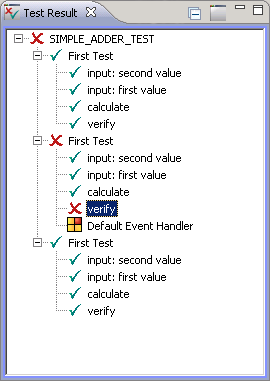
\includegraphics{Tasks/Testexecution/PS/testresultview}
\caption{\gdtestresultview}
\label{testresultview}
\end{center}
\end{figure} 



  

